\documentclass[10pt,sigconf]{acmart}
\usepackage[l2tabu,orthodox]{nag}
\usepackage[utf8]{inputenc}
\usepackage[british]{babel}
\usepackage{ifpdf}
\usepackage{amsmath}
\usepackage[all]{onlyamsmath}
\usepackage{upquote}
\usepackage{graphicx}
\usepackage{url}
\usepackage[caption=false]{subfig}
\usepackage{booktabs}
\usepackage{bytefield}
\usepackage{listings}
\usepackage{algorithm}
\usepackage{algpseudocode}
\usepackage{fancyvrb}
\usepackage{alltt}
\usepackage{color}
\usepackage{balance}
\frenchspacing
\newcommand{\todo}[1]{\textbf{\textcolor{red}{To do: #1}}}
%==================================================================================================
\begin{document}
\title{Describing and Parsing QUIC Packets}

\author{Stephen McQuistin}
\orcid{0000-0002-0616-2532}
\affiliation{%
  \institution{University of Glasgow}
  \streetaddress{School of Computing Science}
  \city{Glasgow}
  \postcode{G12 8QQ}
  \country{UK}
}
\email{sm@smcquistin.uk}

\author{Colin Perkins}
\orcid{0000-0002-3404-8964}
\affiliation{%
  \institution{University of Glasgow}
  \streetaddress{School of Computing Science}
  \city{Glasgow}
  \postcode{G12 8QQ}
  \country{UK}
}
\email{csp@csperkins.org}

\acmYear{2018}
\copyrightyear{2018}
\setcopyright{acmcopyright}
\acmConference{CoNEXT '18}{December 4--7, 2018}{Heraklion/Crete, Greece}
\acmDOI{TBA}
\acmISBN{TBA}
%==================================================================================================
\begin{abstract}

% Four sentences:
%  - State the problem
%  - Say why it's an interesting problem
%  - Say what your solution achieves
%  - Say what follows from your solution

  Standards documents have been slow to adopt formalisms for specifying
  packet formats that go beyond the limited syntax that can be captured
  in ASCII packet diagrams. 
  As increasingly complex protocols, including QUIC, are standardised,
  this is becoming problematic, with descriptions of packet formats being
  fragmented, incomplete, and difficult to follow.
  Further, it is typically not possible to automatically extract parsing
  code from the protocol specification.
  The result is likely to be buggy implementations that do not conform
  to the specification.
  We develop the Network Packet Representation, an abstract, intermediate
  representation that fully captures the syntax of packet formats, and
  that can be generated from a range of packet description languages,
  and can be used to generate packet parsers.
  By specifying an intermediate representation that can be generated from
  both existing and newly developed packet descriptions, we hope to
  encourage the adoption and use of more expressive, machine readable,
  packet descriptions in protocol standards.
  We describe how the Network Packet Representation can be applied to
  the definition of QUIC packets -- the eventual goal being to allow QUIC
  parsers to be automatically generated from the specification.

\end{abstract}
\maketitle
%==================================================================================================
\section{Introduction}

% A good paper introduction is fairly formulaic. If you follow a simple set
% of rules, you can write a very good introduction. The following outline can
% be varied. For example, you can use two paragraphs instead of one, or you
% can place more emphasis on one aspect of the intro than another. But in all
% cases, all of the points below need to be covered in an introduction, and
% in most papers, you don't need to cover anything more in an introduction.
%
% Paragraph 1: Motivation. At a high level, what is the problem area you
% are working in and why is it important? It is important to set the larger
% context here. Why is the problem of interest and importance to the larger
% community?

ASCII packet header diagrams are the most common formalism found in IETF standards
documents. These diagrams allow for the visualisation of packet formats, reducing human error
by aiding in the implementation of protocol parsers. However, while ASCII diagrams can
capture much of the syntax of existing protocols, like TCP and UDP, the complexity
introduced by newer protocols, such as QUIC \cite{draft-ietf-quic-transport-latest},
diminishes their utility. As a result, correct parser implementations are much more
reliant upon the careful interpretation of prose descriptions of the protocol's syntax.
This is a situation that is likely to result in buggy and non-conformant parser implementations.

% Paragraph 2: What is the specific problem considered in this paper? This
% paragraph narrows down the topic area of the paper. In the first
% paragraph you have established general context and importance. Here you
% establish specific context and background.

There are two broad issues with previous efforts to develop formalisms that better capture
the syntax of protocols. Firstly, most are largely unsuitable for protocols like QUIC.
QUIC uses encryption primitives throughout, including protected payloads. This means that
decryption must be modelled. Prior work, which has largely focussed on the parsing of
individual unencrypted packets, is unable to model this. As a result, QUIC, and the broader
shift towards pervasive encryption \cite{rfc7258}, require a new formalism.

The second issue with existing approaches is that they generally define a new language
that standards authors must use to specify their protocols. This limits their adoption:
different documents are suited to different formalisms. As a result,
any approach that is likely to be adopted must be flexible in the input formats that can
be used.

% Paragraph 3: "In this paper, we show that...". This is the key paragraph
% in the introduction - you summarize, in one paragraph, what are the main
% contributions of your paper, given the context established in paragraphs 
% 1 and 2. What's the general approach taken? Why are the specific results
% significant? The story is not what you did, but rather:
%  - what you show, new ideas, new insights
%  - why interesting, important?
% State your contributions: these drive the entire paper.  Contributions
% should be refutable claims, not vague generic statements.

In this paper, we describe a framework for formalising the description of packet formats.
Our framework is comprised of three components: an input parser, an intermediary
representation (the Network Packet Representation), and an output formatter. This
architecture allows packets to be described using a number of different formats, and for
these descriptions to be parsed into a common intermediate form. Output formatters can then
use this intermediate representation to generate various artefacts, including parser code.
We provide an example of how this framework can be used to model the complexity of parsing
QUIC.

% Paragraph 4: What are the differences between your work, and what others
% have done? Keep this at a high level, as you can refer to future sections
% where specific details and differences will be given, but it is important
% for the reader to know what is new about this work compared to other work
% in the area.

There have been many previous attempts at defining a packet format definition language,
including PacketTypes \cite{mccann2000packet}, Melange \cite{madhavapeddy2007melange},
PADS \cite{fisher2005pads}, and DataScript \cite{back2002datascript}. These languages
typically focus on the parsing of individual, unencrypted packets. Ad-hoc languages, such
as the presentation language used in the TLS 1.3 specification
\cite{draft-ietf-tls-tls13-28}, also see limited adoption. In contrast to these language
definitions, in this paper we develop an abstract protocol representation that, with
\emph{contexts} and \emph{functions} can describe the parsing of any protocol, and can be
generated from existing formalisms.

% Paragraph 5: "We structure the remainder of this paper as follows." Give
% the reader a road-map for the rest of the paper. Try to avoid redundant
% phrasing, "In Section 2, In section 3, ..., In Section 4, ... ", etc.

We structure the remainder of this paper as follows. Section \ref{sec:motivation} expands
on our motivation, by assessing the utility provided by an ASCII diagram from the QUIC
standards documents, and outlining the requirements of our formalism. Section
\ref{sec:npr} describes our proposed framework for describing packet formats,
including our intermediary representation, the Network Packet Representation. Section
\ref{sec:casestudy} provides an example of how our framework can be used to capture
the parsing of QUIC's protocol data units (PDUs). Finally, Section \ref{sec:related} discusses
related work, and Section \ref{sec:conclusion} concludes.

%==================================================================================================
% Concentrate single-mindedly on a narrative that:
%  - Describes the problem, and why it's interesting
%  - Describes your idea
%  - Defends your idea, showing how it solves the problem, and filling out
%    the details
% On the way, cite relevant work in passing, but defer discussion to the
% end.
%
% Introduce the problem, and your idea, using examples, and only then
% present the general case. Explain the idea as if your were speaking to
% someone using a whiteboard. Conveying the intuition is primary; details
% follow. Write in a top down manner: state broad themes and ideas first,
% then go into details.
%
% The introduction makes claims. The body of the paper provides evidence
% to support each claim. Check each claim in the introduction, identify
% the evidence, and forward-reference it from the claim. 
%==================================================================================================

\section{Motivation \& Requirements}
\label{sec:motivation}

\begin{figure}
	\centering
	\vspace{3mm}
    \begin{BVerbatim}[fontsize=\scriptsize]
 0                   1                   2                   3
 0 1 2 3 4 5 6 7 8 9 0 1 2 3 4 5 6 7 8 9 0 1 2 3 4 5 6 7 8 9 0 1
+-+-+-+-+-+-+-+-+
|0|K|1|1|0|R R R|
+-+-+-+-+-+-+-+-+-+-+-+-+-+-+-+-+-+-+-+-+-+-+-+-+-+-+-+-+-+-+-+-+
|                Destination Connection ID (0..144)           ...
+-+-+-+-+-+-+-+-+-+-+-+-+-+-+-+-+-+-+-+-+-+-+-+-+-+-+-+-+-+-+-+-+
|                      Packet Number (8/16/32)                ...
+-+-+-+-+-+-+-+-+-+-+-+-+-+-+-+-+-+-+-+-+-+-+-+-+-+-+-+-+-+-+-+-+
|                     Protected Payload (*)                   ...
+-+-+-+-+-+-+-+-+-+-+-+-+-+-+-+-+-+-+-+-+-+-+-+-+-+-+-+-+-+-+-+-+
    \end{BVerbatim}
    \caption{QUIC short header format (from \cite{draft-ietf-quic-transport-latest})}
    \label{fig:quic-short-hdr}
\end{figure}

Broadly, the requirements for our formalism are that it should:
\begin{itemize}
	\item be able to fully capture the information required for \emph{parsing} PDUs;
	\item accommodate various PDU specification languages, including ASCII
		  packet header diagrams, ad-hoc languages
		  such as the TLS 1.3 presentation formation, and more generic packet description
		  languages;
	\item produce output in a number of formats, including ASCII diagrams, and parser
		  code.
\end{itemize}

To demonstrate the limitations of ASCII packet header diagrams in capturing all of the
information required to fully parse PDUs, we consider the diagram for QUIC's short header
PDU, as shown in Figure \ref{fig:quic-short-hdr}. From this diagram, it is clear how the
first octet should be parsed: the widths of each field are known, and, for some, the
values specified. However, it is not clear how the Destination Connection ID, Packet
Number, and Protected Payload fields should be parsed. Determining the syntax
of these fields requires the prose descriptions that accompany the diagram: the
expressivity of ASCII packet diagrams is limited.

Some of these limitations can be overcome by using an existing packet
description language. Such languages typically allow for intricate field encodings to be
specified. For example, packet numbers use a variable-length integer encoding format,
where the most significant bits of the first octet determine the length of the field.
While it is impractical to represent this behaviour in an ASCII diagram, most packet
description languages enable this format to be captured.

However, we have identified two broad features that are missing from existing packet
description languages that mean that they cannot capture the behaviour of all 
protocols, including QUIC, where
encryption is part of the parsing process, or RTP, where PDUs cannot be parsed discretely.

Firstly, existing languages typically enable per-packet modelling, but decryption in QUIC
requires information from packets earlier in the flow. We require flow-level
\emph{context}: essentially a key-value store that can be added to as parsing progresses,
and modelled as part of the protocol specification. For example, the nonce for decrypting
the protected payload field is derived from the packet number. However, the packet only
contains the least significant bits of this number. Contextual information from other
packets in the flow is required to generate the nonce. As an additional example where 
contextual information is required for parsing, we consider RTP \cite{RFC3550}. RTP
includes support for header extensions, whose format is signalled out-of-band using SDP;
context is needed to share information between different parsing events, and out-of-band
processes.

The second feature needed to fully model the parsing of QUIC is the ability to capture
\emph{how} encrypted fields are parsed. Existing description
languages have been able to treat encrypted fields as unparsable blobs, enabled by the
separation between protocols. For example, where TCP is used to carry an encrypted
payload, the format of the payload is not specified as part of TCP: the parsing of TCP can
end with the payload as an encrypted blob. However, in QUIC, parsing a short header packet
requires that the protected payload by decrypted, and further parsed into frames. As a
result, we must model the \emph{functions} required in the parsing of the protocol.

To fulfil our second two requirements -- flexibility in both input and output formats --
our formalism must be an abstract, intermediate representation language. Such a
representation can be generated from an arbitrary set of input formats, and can itself be
used to produce various outputs. This allows for existing formalisms, including ASCII
packet diagrams and the TLS 1.3 presentation language, to be used. The expressivity
of the intermediate representation depends on the input format; this allows for adoption
while incentivising more expressive formalisms.

%==================================================================================================
\section{Describing Protocol Data}
\label{sec:npr}

We introduce the Network Packet Representation, a type system the allows
the format of protocol data units to be specified, alongside information
on how those PDUs should be parsed.
Key to this is the definition of a type system (\S\ref{sec:npr-types}) that
describes the format of PDUs, helper functions, and the context needed for
parsing.
This is associated with one or more protocol description languages
(\S\ref{sec:npr-input}) that describe the PDUs to be parsed; and one
or more parser generators (\S\ref{sec:npr-output}) that can generate
implementations of parsers for those PDUs.
These components are illustrated in Figure \ref{fig:stages}.

\begin{figure}
  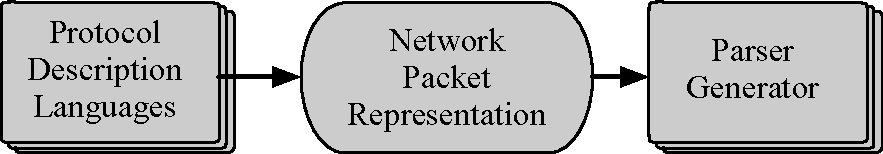
\includegraphics[width=\linewidth]{figures/architecture-flow.pdf}
  \caption{Describing, representing, and parsing PDUs}
  \label{fig:stages}
\end{figure}

%--------------------------------------------------------------------------------------------------
\subsection{A Type System for Protocol Data}
\label{sec:npr-types}

The Network Packet Representation type system describes the format of PDUs,
along with the helper functions and context needed to parse them.

The base type class used to describe PDUs is a \emph{Bit String}.
This is a sequence of $n$ consecutive bits of data that can be instantiated
as a named type.
For example, a type system to describe RTP \cite{RFC3550} might instantiate
a new instance of the bit string type class, \texttt{SeqNum}, comprising 16
bits to represent an RTP sequence number.

There are three classes of derived types that represent structured data in
a PDU: array types, structure types, and enumerated types.
An \emph{Array Type} represents a sequence of values of some other type; 
it may have fixed or unspecified length. If the length is unspecified in
the definition of the array type, it must be possible to infer it based
on the constraints of an enclosing structure type, discussed below.

A \emph{Structure Type} represents a heterogeneous collection of fields.
They are the main types used to represent complex packet formats.
At a high-level, structure type definitions resemble those in programming
languages such as C: they comprise a sequence of fields, each with its own
type, that are packed together in the order specified. Unlike C, no padding
can be present between fields, and the size of all types is well-defined
and derived from the size of the underlying bit string types (there is no
undefined or implementation defined behaviour).

Structure types represent protocol data that can be parsed.
For example, a QUIC frame, or a TCP header.
The format of a particular instance of a structure type, as it is parsed,
is determined by a set of constraints on the fields that structure, and
transformations of those fields. 
There are two types of \emph{Constraint Expression} that can affect parsing
of a structure instance: \emph{is\_present} constraints on specific fields,
and structure-level constraints.
The former are attached to optional fields, and are boolean expressions
that declaratively indicates whether those fields are present when the
structure is parsed.
The latter are attached to the structure as a whole, and specify more
complex constraints, potentially across multiple fields, that must hold
for the packet to be valid when parsed. 
Constraint expressions can reference the values of fields of the enclosing
structure, methods defined on those fields, fields in the parsing context,
or helper functions. 
For example... \todo{add constraint example}

The \emph{Parsing Context} allows the parser to keep state between packets.
It is essential to parsing complex protocols, and the ability to specify
data to be stored in the context is one of the key innovations of our
Network Packet Representation.
Typical uses of the parsing context include:
1) recording the cryptographic keys and other information relating to the
   security context;
2) storing parameters set in early packets, to allow parsing of later 
   packets; and
3) storing parameters specified in out-of-band signalling, that are 
   needed to parse packets (e.g., in the context of RTP, signalled
   payload type values or the meanings of header extensions \cite{RFC5285}).
Structure types can also be tagged with a series of \emph{Actions} that are
performed when they are parsed.
The actions are generally expressed in terms of calls to helper functions
that update the parsing context.

The Network Packet Representation allows the definitions of \emph{Function
Prototypes}. These can be either \emph{Helper Functions} or \emph{Transform
Functions}.
The function prototypes specify the function name, parameter names and types,
and the return type only; they do not specify the body -- the Network Packet
Representation is a type system not a complete programming language.
Helper functions specify constraints or actions; transform functions define
how a field is processed after parsing to generate a replacement field.
A common example of the latter might be a \texttt{decrypt()} function that
takes a key previously stored in the parsing context (e.g., by a call to an
action function specified on parsing of an initial handshake packet) to
decrypt a protected payload field.  The intent is that the semantics of the
function are specified in prose, in the protocol specification, while its
arguments and return type are specified in the input protocol description
language (see Section \ref{sec:npr-input}).
Together, constraint expressions and transform functions allow structure
types to represent complex PDU formats, such as those used in QUIC.

\emph{Enumerated Types} allow specification of alternatives: a PDU can
be either s PDU of type \emph{X} or type \emph{Y}. Finally, the overall
\emph{Protocol Type} includes definitions for the other types, and gives
the types of the PDUs used in the protocol.


The type system of the Network Packet Representation is supported by an
\emph{intermediate representation}; a well-defined serialisation format
that can be generated from the front-end protocol description languages
and used to instantiate the types describing the protocol data.


% The runtime defines a set of primitive types that can be parsed or serialised (that is,
% they are \emph{representable}):
% \begin{itemize}
% 	\item Bit string
% 	\item Array
% 	\item Structure 
% 	\item Variant
% 	\item Function
% 	\item Protocol
% 	\item Context
% \end{itemize}

% Types are formed both by the types of value they can hold, and the \emph{traits} that they
% implement. Traits define the methods that can be used on the types. The protocol type is
% the top-level type of the intermediate representation; it contains the constructors for
% the protocol-specific types, and lists the PDUs that comprise the protocol. We omit
% discussion of the bit string, array, and variant types: these are intuitive, and broadly
% match with traditional definitions.

% The structure type also largely matches its widely used definition.
% However, we augment the typical C-style composite type in two important ways. Firstly, each field of
% the structure can be associated with a \emph{transformation}: this captures if, and how,
% the field changes after it has been parsed. For example, in QUIC, payloads are protected:
% the payload field begins with an encrypted bit string type, and after parsing, is
% transformed into a field with that is an array of frames. Importantly, these
% transformations are needed in the parsing process: parsing of a PDU would not be complete
% without decrypting the protected payload. Secondly, structures have a set of constraints:
% expressions that define structures by limiting the values that their fields can hold. For
% example, a structure might have the same layout as another, but differ on the value of a
% particular field.

% The function type holds the signature of external helper functions, and consists of the
% function's name, parameters (their name and type), and return type. The body of the
% function is \emph{not} captured. As described above, functions are necessary when
% modelling the parsing process.

% The context type defines the variables (their name and type) that can be accessed in the
% parsing of PDUs, by helper functions, or out-of-band (e.g., in code that handles PDU
% serialisation). The context holds the internal state for the parser: it is used to store
% data that is necessary for parsing to progress.

% In addition to these representable types, the runtime also has a number of \emph{internal}
% types: these are types that are used within the runtime, but that cannot be parsed or
% serialised. These are intuitive, and include booleans and integers.

%--------------------------------------------------------------------------------------------------
% \subsection{Intermediate representation}
% \label{sec:gpl-ir}

% The runtime defines a constructor for each of the representable types described in the
% previous section. These constructors instantiate new types derived from the parameterised
% base type. For example, a constructor might be used to construct a 16-bit bit string, with
% the name \emph{Int16}. \emph{Int16} then becomes a type that can be used throughout the
% intermediate representation. Derived types can also be further defined by implementing
% additional traits. For example, \emph{Int16} could implement ordinal and boolean traits to
% make it an integer type.

% The high-level object of the intermediary representation is a protocol object; exactly
% one protocol type must be constructed. The protocol object then contains a list of
% constructors for the other types instantiated. With the exception of the context type,
% any number of constructors may be defined; at most one context can be constructed, given
% its nature. Finally, the protocol type includes a list of the PDUs that comprise the
% protocol, based on the constructed types.

% The intermediate representation is serialised using JSON. By using a widely adopted
% notation, the code used to both generate the representation, and use it, is not tied to a
% particular programming language. The role of the intermediate representation is to join
% together two arbitrary programs: one that generates it, and another that uses it to
% produce output, such as a parser.

% This means that the Network Packet Representation differs from previous work in this area:
% protocol designers do not formalise their specifications using the language itself, but
% rather, they use whichever formalism is appropriate, and develop tooling around that. For
% example, the QUIC protocol documents make use of ASCII packet diagrams and the TLS 1.3
% presentation language. Tooling can be developed to parse these existing formalisms from
% the documents, and to generate the intermediate representation. This approach fits better
% with the standardisation process used in bodies like the IETF: prior efforts to introduce
% formalisms have largely failed because of their expectation that protocol authors must
% change how they write specifications. The Network Packet Representation's intermediate
% representation can be generated from any formalism, but the level of detail captured
% varies with the expressiveness of that formalism.

% The same flexibility in how the intermediate representation is generated also applies to
% how it can be used to derive output formats: any program that can interpret the JSON
% format can read the intermediate representation can generate output from it. There are
% obvious use cases, such as generating ASCII packet diagrams or stubbing out parsers in C.
% But ultimately, the benefit of the approach here is that the output is not coupled to the
% input format: code that takes the intermediate representation and generates a C parser can
% be written once, and reused regardless of how the intermediate representation was
% generated.

% An additional benefit to having a common intermediate representation is that tooling can
% be developed around it, without duplicated effort. Such tooling could type check the
% intermediate representation, to ensure that it had been generated correctly.

%--------------------------------------------------------------------------------------------------
\subsection{Protocol Description Languages}
\label{sec:npr-input}

The intermediate representation that is used to construct the Network Packet
Representation is generated by programs that parse a protocol description language, rather
than by standards authors. This decoupling means that \emph{any} protocol description
language can be used, including ad-hoc, domain-specific languages. This is in contrast to
previous approaches, where all documents were expected to adopt a common description
language.

The flexibility of this approach means that the definition of a protocol description
language can be broad, ranging from ASCII packet diagrams, to the TLS 1.3 presentation
language. Importantly, these languages are already in use: parsers can be written for them
to gain the benefits of having a common representation. As we describe in
Section~\ref{sec:related}, many description languages have been already been defined;
these too can be used to generate the intermediate representation.

Building a parser for an existing language allows for widespread adoption of the Network
Packet Representation, and enables the benefits that come with having a common
representation. However, a key motivation for the representation is that existing
languages cannot model features of common protocols. The expressiveness of the language
used to generate the intermediate representation determines how well the protocol is
defined. For example, ASCII packet diagrams do not allow for relationships between fields
to be defined; these would then be missing from the intermediate representation. As a
result, the use of existing languages can be viewed as a transitional phase: as the
benefits of a common representation become clearer, more expressive languages can be
adopted as part of the standardisation process. We use one such language as part of our
QUIC example in Section~\ref{sec:casestudy}.

%--------------------------------------------------------------------------------------------------
\subsection{Parser Generators}
\label{sec:npr-output}

Once the intermediate representation has been produced, it can be used to generate a
parser for the protocol that it describes. Again, the flexibility of having a common
representation means that a parser can be generated for \emph{any} target language, such
as C or Rust. Previous approaches would have required writing a parser generator for each
protocol description language: decoupling these components means that only one parser
generator needs to be written for each target language.

Commonality in \emph{how} parser generators are created means that tooling can be used to
support their development. For example, in many target languages, the order in which types
need to be defined is the same. Tooling could implement this logic once, easing the
development of parser generators.

There are two main benefits that are derived from generating parsers from a common
intermediate representation. Firstly, the parsers that are generated will be compliant
with the described protocol, and are less likely to introduce bugs. In addition, once a
parser generator has been written, parsers can be generated in novel, safe languages, such
as Rust \cite{chifflier2017writing}, without additional effort.

%==================================================================================================
\section{Example: Parsing QUIC}
\label{sec:casestudy}

\begin{figure}
	\vspace{3mm}
    \begin{BVerbatim}[fontsize=\scriptsize]
VarInt := {
	two_bit       : Bit2;
	value         : Bits;
} where {
	value.length == (8*(2^two_bit))-2;
};

PacketNumber7 := {
	first_bit     : Bit;
	packet_number : Bit7;
} where {
	first_bit == 0;
};

PacketNumber14 := {
	first_twobits : Bit2;
	packet_number : Bit14;
} where {
	first_twobits == 1;
};

PacketNumber30 := {
	first_twobits : Bit2;
	packet_number : Bit30;
} where {
	first_twobits == 2;
};

PacketNumber := { PacketNumber8 | PacketNumber16 | PacketNumber32 };
                     
Context := {
	highest_packet_num  : PacketNum;
	last_scid           : ConnectionID;
};
    \end{BVerbatim}
    \caption{Complex data types for QUIC parsing}
    \label{fig:quic-base}
\end{figure}

\begin{figure}
	\vspace{3mm}
    \begin{BVerbatim}[fontsize=\scriptsize]
lh_packetnum_decrypt :: (ppacket_num : Bits, 
                         context : Context) 
                     -> PacketNum;

LongHeader := {
	header_form   : Bit;
	packet_type   : Bit7;
	version       : Bit32;
	dcil          : Bit4;
	scil          : Bit4;
	dcid          : Bits;
	scid          : Bits;
	length        : VarInt;
	ppacket_num   : Bits -> packet_num : PacketNum;
	payload       : Frame[];
} where {
	header_form == 1;
	dcid.size == ((dcil == 0) ? 0 : dcil+3);
	scid.size == ((scil == 0) ? 0 : scil+3);
} onparse {
	packet_num = lh_packetnum_decrypt(ppacket_num, Context);
	Context.packet_num = packet_num;
};
    \end{BVerbatim}
    \caption{QUIC long header (from \cite{draft-ietf-quic-transport-latest})}
    \label{fig:quic-long-hdr-desc}
\end{figure}

In this section, we will demonstrate that the novel features of the Network Packet Representation
 -- functions and context -- are necessary in describing QUIC. We illustrate
this using an example that formalises some of QUIC's PDUs using a protocol description
language. As discussed in the previous section, this language itself is not important: the
Glasgow Packet Representation is agnostic to input and output formats. The syntax the
language we use here has been designed to demonstrate the functionality provided by the
intermediate representation. Finally, the examples used in this section are not exhaustive:
for example, we look at the long and short header packet formats, and how their parsing
can be modelled. We do not consider packet-level protection (e.g., 0-RTT protection for
long header packets), but this does not limit the generality of our approach.

We begin, in Figure~\ref{fig:quic-long-hdr-desc}, by describing QUIC's long header
format. This code declares a \texttt{LongHeader} type, a structure with the fields as
specified in the first block. The \texttt{Bit} and \texttt{Bit\emph{N}} types are instances
of the bit string type, with sizes 1 and \emph{N} respectively. The complex data types 
used in the \texttt{LongHeader} structure are defined in Figure~\ref{fig:quic-base}. The
\texttt{VarInt} type is a structure that encapsulates QUIC's variable-length integer
encoding format. \texttt{PacketNum} encodes the similar variable-length packet number
format as a variant type, where the variants depend on the first one or two bits of the
format to determine the width of the packet number.

The \texttt{where} block further defines the \texttt{LongHeader} type, by constraining the
values that the structure's fields can take. A PDU is a \texttt{LongHeader} type only if
all of the constraints in the \texttt{where} block are true. This highlights the benefit
of this programmatic description of the long header: the relationship
between the \texttt{dcil}/\texttt{scil} and \texttt{dcid}/\texttt{scid} fields is made
explicit. In the standards documents, where ASCII packet diagrams are used, the
\texttt{dcid}/\texttt{scid} fields are shown as having variable lengths; the prose
description accompanying the diagram is needed to fully describe the packet format.

The \texttt{onparse} block contains actions that are to be performed once the PDU has been
successfully parsed as a \texttt{LongHeader} type (i.e., its layout matches that of
the structure, and all of the constraints in the \texttt{where} block are true). The
\texttt{onparse} block introduces an imperative element into an otherwise declarative type
definition. The actions listed in the \texttt{onparse} block, and captured by the intermediate
representation, are not intrinsic to the \texttt{LongHeader} type: they are expressions that
allow the parsing process to progress.

The
single expression in this section is matched with the following field of the structure:
\footnotesize
\begin{alltt}
    ppacket_num : PPacketNum -> packet_num : PacketNum
\end{alltt}
\normalsize
This is a field transformation: it indicates that the parsed block
contains a protected packet number field (with type \texttt{Bits}), which, to allow
for further parsing, is then transformed (using the \texttt{lh\_packetnum\_decrypt} function)
into a packet number field (with type \texttt{PacketNum}). The intermediate
representation captures the signature of the functions required in the parsing of the
protocol. At present, much of this behaviour is captured in prose descriptions of the
protocol, limiting the usefulness of the ASCII packet diagrams the documents provide.
This issue is exacerbated by the TLS-related functionality being described in a separate
document (e.g., packet number protection is described in Section 5.3 of the
QUIC-TLS draft \cite{draft-ietf-quic-tls-14}). Using explicit function names would provide
a concrete way of linking these components together. 

Finally, Figure~\ref{fig:quic-long-hdr-desc} makes use of the \texttt{Context} type,
defined in Figure~\ref{fig:quic-base}. As
described in the previous section, the context is essentially a key-value store. Type
declarations can access the context, to check against values that it contains, and actions,
functions, and out-of-band processes can access and change values in the context. In
this example, the context includes a \texttt{highest\_packet\_num} field. The field
transformation captures that the
\texttt{lh\_packetnum\_decrypt} function removes the packet
number protection, and decodes the truncated packet number into the full packet number.
The decoding process requires not only the truncated packet number (i.e., the unprotected
incoming packet number), but also the largest packet number seen so far. As shown, this is
stored in the context, which the \texttt{lh\_packetnum\_decrypt} function can access.

\begin{figure}
	\vspace{3mm}
    \begin{BVerbatim}[fontsize=\scriptsize]
decrypt :: (ppayload : Bits, 
            context : Context) 
        -> Frame[];

sh_packetnum_decrypt :: (ppacket_num : Bits, 
                         context : Context) 
                     -> PacketNum;
                     
ShortHeader := {
	header_form   : Bit;
	key_phase     : Bit;
	third_bit     : Bit;
	forth_bit     : Bit;
	demux_bit     : Bit;
	reserved      : Bit[3];
	dcid          : Bits;
	ppacket_num   : Bits -> packet_num : PacketNum;
	ppayload      : Bits -> payload : Frame[];
} where {
	header_form == 0;
	third_bit == 1;
	forth_bit == 1;
	demux_bit == 0;
	dcid == Context.scid;
} onparse {
	packet_num = sh_packetnum_decrypt(ppacket_num, Context);
	Context.packet_num = ((packet_num > Context.packet_num)
	                        ? packet_num 
	                        : Context.packet_num);
	payload = decrypt(ppayload);
};
    \end{BVerbatim}
    \caption{QUIC short header (from \cite{draft-ietf-quic-transport-latest})}
    \label{fig:quic-short-hdr-desc}
\end{figure}

Next, we consider the short header, as shown in Figure~\ref{fig:quic-short-hdr-desc}.
Beyond the features already discussed as part of the long header example, the short header
also includes a reference to the context. The short header's \texttt{dcid} field must
match the most recent source connection ID that has been sent. This demonstrates another
way in which the context can be accessed: the sending process is essentially out-of-band,
but information must be shared with the parsing process to allow it to progress.

\begin{figure}
	\vspace{3mm}
    \begin{BVerbatim}[fontsize=\scriptsize]
PaddingFrame := {
	frame_type   : VarInt;
} where {
	frame_type == 0;
};

Frame := { PaddingFrame | RSTStreamFrame | ConnectionCloseFrame | .. };
    \end{BVerbatim}
    \caption{QUIC frames (from \cite{draft-ietf-quic-transport-latest})}
    \label{fig:quic-frame-desc}
\end{figure}

This is the central argument for requiring helper functions and context: decryption (in
the form of packet and payload protection, for example) are primitives of the QUIC
protocol. If we are to design an intermediate language that can model the parsing of QUIC
PDUs, it \emph{must} allow for the modelling of decryption. This is further illustrated
by the link between the short header format's protected payload, and the QUIC frames (as
shown in Figure~\ref{fig:quic-frame-desc}) that it ultimately contains. It is not sufficient
to treat the protected payload as an encrypted blob: this does not fully model the parsing
process. As shown, a short header PDU is parsed, and the payload is decrypted using the
\texttt{decrypt} function, which takes both the protected payload and the context (for any
information needed to decrypt the payload), and returns an array of frames. The frames are
then parsed as the \texttt{Frame} type defined in Figure~\ref{fig:quic-frame-desc}.

The example given here also hints at the boundary between modelling the parsing of a 
protocol's PDUs, and validating that those PDUs make sense within the broader semantics 
of the protocol. For example, we use enough logic to store the highest packet number seen,
but do not otherwise validate incoming packet numbers. The intermediate representation is
designed to capture only the information that is required to parse PDUs: ultimately, PDUs
might parse successfully, only to be rendered invalid by the semantics of the protocol.

%==================================================================================================
\section{Related Work}
\label{sec:related}

% This should come near the end, and focussing on discussing how your work
% relates to that of others. Any relevant related work should have been
% cited already, so this is not a list of related work, it's a discussion
% of how that work relates.
%
% Why not put related work after the introduction? 1) because describing
% alternative approaches gets between the reader and your idea; and 2)
% because the reader knows nothing about the problem yet, so your
% (carefully trimmed) description of various technical trade-offs is
% absolutely incomprehensible.
% 
% When writing the related work:
%  - Give credit to others where it's due; this doesn't diminish the
%    credit you get from your paper. 
%  - Acknowledge weaknesses in your approach.
%  - Ensure related work is accurate and up-to-date

There have been many previous efforts to develop protocol description languages.
Some, such as PADS (Processing Ad Hoc Data Sources)
\cite{fisher2005pads} and DataScript \cite{back2002datascript}, are C-like in their syntax
and type systems. Others, like PacketTypes \cite{mccann2000packet} and the Meta Packet
Language (MPL) \cite{madhavapeddy2007melange}, are declarative, with more expressive type
systems. None of these approaches include support for contexts or helper functions: there
is no way to model either the decryption primitives that are essential to the parsing of
QUIC, or the out-of-band information needed to parse protocols like RTP.
Ultimately, while these languages are well-motivated (i.e., parser quality
would be improved by formal specifications in standards documents), they
misunderstand the needs of standards authors, and provide no way of
transitioning from existing approaches, to those that they define.

In terms of adoption, it's interesting to consider approaches that see use in IETF
documents. Most widespread is the ASCII packet diagram. While this is
limited in its expressiveness, its value in showing the layout of protocol PDUs should not
be ignored. Other formalisms, such as ASN.1 \cite{x680} and the TLS 1.3 presentation
format \cite{draft-ietf-tls-tls13-28}, see widespread adoption within certain IETF
working groups, but almost no adoption in most. This points to the problem noted above: a
single input language is not suitable in all cases. The flexibility of our approach --
defining a common intermediate representation and type system from which
parsers can be derived, rather than define a single protocol description language
that authors must write -- means that existing formalisms, e.g., ASCII
diagrams and the TLS 1.3 presentation language, can be used as input
formats, with other representations, such as that we outline in Section
\ref{sec:casestudy}, being developed when they become useful. 

The flexibility is also beneficial in terms of the output formats that can be derived.
Beyond the traditional parser languages described in
Section~\ref{sec:npr-output}, we also consider P4
\cite{bosshart:2014:p4,p4consortium:2018:v16spec-20180531}, a language for
programming the data plane of network devices. It is widely used in software defined
networking applications. P4 describes how packets are parsed and serialised and what state
tables exist in a network devices, and specifies a series of match-action rules that
describe the packet processing and forwarding behaviour of the device. Parsers in P4 are
implemented imperatively, and are built-up from a series of state machines. In terms of
expressive power, parsers in P4 are comparable to the parsers we describe and can parse
the same formats. Our approach differs from P4 in that we declaratively define the packet
format, and derive the parser implementation from that declaration. P4, on the other hand,
simply specifies the parser implementation. As such, P4 could be an appropriate output
language for our system.

%==================================================================================================
\section{Conclusions and Future Work}
\label{sec:conclusion}

We have described the Network Packet Representation, a type system that
allows the format and parsing of protocol data units to be described.
This builds on existing approaches in three important ways. First, in
recognising that encryption primitives are a fundamental component of new protocols, we
allow for out-of-band helper functions to be modelled. A related addition is the inclusion
of a persistent (across the parsing process) context, to allow for data to be exchanged
between the parsing of different PDUs, or out-of-band logic. Finally, the representation
defines an intermediate representation that can be generated from any input format, and
can be similarly used to generate output in any format.

% Future work includes development of tooling that allows for the intermediate
% representation to be type checked. This illustrate the benefit of a common intermediate
% representation: the effort required to support a new input or output format is not
% duplicated.

By defining a common type system for protocol data, we aim to provide the
benefits of formal specifications without mandating change to the way that
protocols are currently specified.
Our intermediate representation can be generated by parsing ASCII diagrams
as they are written today, for example.
While this representation would lack the expressiveness of more formal
description (such as the examples in Section \ref{sec:casestudy}), it would
provide some of the benefits, and incentivise authors to move beyond ASCII
diagrams to more sophisticated description formats.
We outline one such format that might be used to define the syntax of QUIC
packets.
We believe that this piecemeal approach fits better with the IETF standards
process: common infrastructure and tooling, but no mandated input format or
output language.

%==================================================================================================
\section*{Acknowledgements}
\footnotesize

This work is funded by the UK Engineering and Physical Sciences Research Council, under
grant EP/R04144X/1.

%==================================================================================================
\balance
\bibliographystyle{ACM-Reference-Format}
\bibliography{improving-quic-docs}
\end{document}
%==================================================================================================
% vim: set ts=2 sw=2 tw=75 et ai:
